\documentclass[article]{aaltoseries}
\usepackage[utf8]{inputenc}
\usepackage{algorithm}
\usepackage{algorithmic}


\begin{document}
 
%=========================================================

\title{Comparison of Three Machine Learning approaches in Image Recognition}

\author{Dongmin Wu
\\\textnormal{\texttt{dongmin.wu@aalto.fi}}
\\
Shan Kuan
\\\textnormal{\texttt{shan.kuan@aalto.fi}}
} % Your Aalto e-mail address

\affiliation{\textbf{Tutor}: Vesa Hirvisalo, Jussi Hanhirova} % First and last name of your tutor

\maketitle

%==========================================================

\pagebreak

%============================================================


\section{Introduction}


Deep learning has been widely used recently. As the main algorithm of Deep learning technology,
the popularity of neural network algorithm 
have considerably increased and become the state-of-the art for solving different pattern recognition
problems.

Neural network is inspired by the neural system of the human brain. A neural network will 
try to model pattern of data by using a large number of intelligent nodes, which are named perceptrons. 
After gathering those computational units together, due to the high complexity of neural networks. 
This algorithm has the potential to fetch non-linear features from the training data 
and build a more precise pattern.

As the result, in the image recognition area, the performance of Deep learning is generally better than
other Machine Learning algorithms.  

In the winter semester of 2017, the group G1-COORD take responsible of a self-driving car project. 
This paper is aim to help the project with choosing an appropriate Deep learning model. The main 
criteria is the accuracy of the prediction, in addition, the inference time will be another 
parameter.

This paper will firstly introduces the background of Deep neural network and the characteristic of it in section \ref{sec:background}.
We find three possible approaches for deep learning algorithm and will list them in section \ref{sec:approaches}.
The section \ref{sec:experiment} shows our experiments among those three approaches.
Finally, in the section \ref{sec:conclusion}, we will give the conclusion based on our experiments.






%============================================================


\section{Background}
\label{sec:background}

In this section, a brief introduction of Deep learning. Those fundamental 
knowledge helps us to understand the context of this paper better.


%------------------------------------------------------------


\subsection{Deep Learning and neural network}

The neural network in Deep learning can be called Deep Neural Network(DNN), which is one of the most promising 
part of current machine learning methods. 

\subsubsection{History of Deep Neural Network}

% 1. history  1page
Back to middle 1900's there is already a paper introduced a Artificial Neural Network (ANN)\cite{Warren1943}, authors
of that paper raise up the first shallow ANN which mimics the neural network system of human brain. That ANN are not
able to learn models from data, but following researches extended the capabilities of ANN and generated unsupervised 
learning algorithm and supervised algorithm subsequently.

In the 1970s and 1980s, back-propagation learning algorithm was found. Because of efficiency the application of back-propagation
reached its peak in the middle of 80's. LeCun applied this algorithm on the convolutional neural network 
for the first time on 1989, which has significant impact to the Deep learning area. After that, the Cresceptron Model was introduced
and the using of max-pooling layers in the neural network architecture was widely used in modern Deep learning technology.

After the year of 2010, Deep learning has another wave of popularity because there are more affordable GPUs with powerful 
parallel computation capacities. AlexNet\cite{NIPS2012_4824} earned the first prize of 
the 2012 ImageNet Large-Scale Visual Recognition Challenge (ILSVRC). 

From then on, the researching of DNN was considerably accelerated. Google, Facebook, Apple and Amazon has beed published
their own papers in this area. In 2015, Google introduced their GoogLeNet\cite{GoogLeNet}, whose Inception model composing the convolutional 
neural network in a new way that no sequentially arranged layers are possible. In the same year, the ResNet\cite{ResNet} of Microsoft won 
the ILSVRC with the error rate of 3.6\%, which is empirically smaller than the error rate of human beings.




\subsubsection{Characteristic of Deep Neural Network}
% 2. characteristic 1page

The Deep Neural Network higher hierarchy than ANNs, which means a large amount of hidden layers\cite{MAL-006}. 
That difference makes DNN can understand more complex model than ANN, which means the Deep learning or especially DNN
has better behavior on describing non-linear objects, including image, voice, text and bioinformatics.

Besides, comparing to Machine learning technology, deep learning are more suitable for various tasks. The basic concept
of DNN is multi-layers neural network, that algorithm will produce pattern by itself only rely on a large data set
, on the contrary side of some algorithms specifically designed for tasks. With DNN technology, users can tackle different
issue with one implementation of DNN. 

As the widely using of Big data technology, the old machine learning technologies like Support Vector Machine (SVM) are
not such suitable for processing a large amount of data. On the other hand, because of the discovering of back-propagation
algorithm, the efficiency of DNN is relatively higher than traditional Machine learning algorithms.

DNN is more flexible as well. Since the DNN is consisted by multiple neutrons, the amount of neutrons can be adjusted
according to the requirement of different task. This characteristic made DNN has large potential of applying. So far, 
DNN have already impacted our life, services like Google translate, AlphaGo and Siri are the examples of successful applications.


\section{Three approaches of Deep Neural Network}
\label{sec:approaches}

\subsection{Softmax Regression}



Softmax Regression(or Multi-class Logistic Regression) is a generalization of logistic regression 
that we can use for multi-class classification.
The softmax regression is an extending of Logistic Regression model which can only perform binary classification tasks.

The equation \ref{eq:softmax} is the mathematic form of softmax function. Softmax function will produce values from 0 to 1
and ensure the sum of them equals to 1. 

\begin{equation}
\label{eq:softmax}
 P(y=j|z^{(i)} )= \phi_{softmax} (z^{(i)}) = \frac{ e ^{z^{(i)}}}{\sum_{j=0}^k e ^{z^{(i)}}}  
\end{equation}

The architecture of softmax regression is shown in Figure \ref{fig:softmax_regression}. 
The cross-entropy function\cite{crossEntropy2005} performs as the cost function of the neural network.

\begin{figure}[t!]
  \begin{center}
    % Note how the file extension has been removed from the filename below
    % so that the LaTeX command can automatically pick any supported file format
    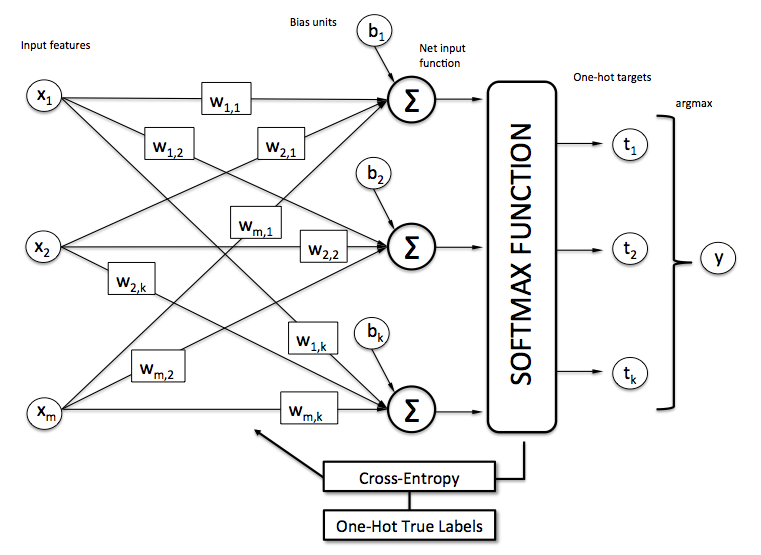
\includegraphics[width=0.8\textwidth]{figures/softmax_regression_schematic}
    \caption{A softmax regression with cross-entropy as the cost function.}
    \label{fig:softmax_regression}
  \end{center}
\end{figure}


\subsection{Feed-Forward Neural Network}

In 1943, McCulloch et al. published a paper\cite{mcculloch1943logical}, tried to understand how the brain could 
produce highly complex patterns by using many basic cells that are connected together.

After years evolution, the feed-forward neural network are able to solve the non-linear problems within replace
the original sign function with non-linear activation functions like sigmoid and tanh.

Figure \ref{fig:feed_forward} shows a typical architecture of feed-forward neural network. The feed-forward neural
network could be treated as a extended version of softmax regression, along with the increasing number of hidden layers, 
the network is able to handle with more complex problems.

\begin{figure}[t!]
  \begin{center}
    % Note how the file extension has been removed from the filename below
    % so that the LaTeX command can automatically pick any supported file format
    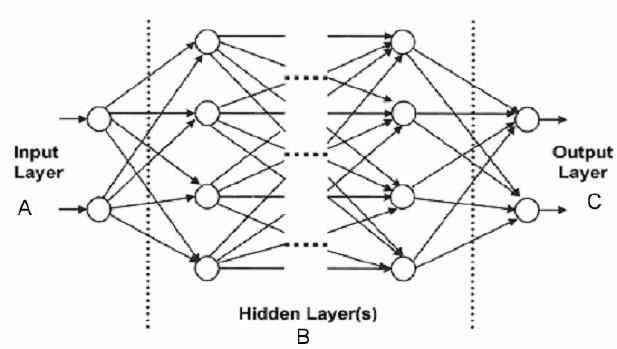
\includegraphics[width=0.8\textwidth]{figures/feedforward_neural_network}
    \caption{A typical feed-forward neural network has three type of layers: input layer, hidden layers and output layer.}
    \label{fig:feed_forward}
  \end{center}
\end{figure}

\subsection{Convolutional Neural Network}

Convolutional Neural Network(CNN) is another upgrading of feed-forward neural network, the network consist of 
convolutional layers, pooling layers, fully connected layers and normalization layers.

Convolutional layers will compute the output of neurons that are connected to local regions in the input, 
each computing a dot product between their weights and a small region they are connected to in the input volume. 

Pooling layer will perform a downsampling operation along the spatial dimensions (width, height)

Fully connected layer is a traditional Multi Layer Perceptron that uses a softmax function in the output layer.

Figure \ref{fig:leNet} is the architecture we used in this paper.


\begin{figure}[t!]
  \begin{center}
    % Note how the file extension has been removed from the filename below
    % so that the LaTeX command can automatically pick any supported file format
    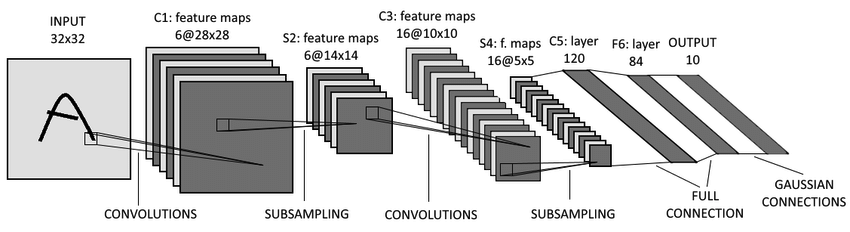
\includegraphics[width=1\textwidth]{figures/LeNet-5}
    \caption{A LeNet-5 convolutional neural network designed by LeCun et al.\cite{lecun1998gradient}.}
    \label{fig:leNet}
  \end{center}
\end{figure}

\section{Experiment}
\label{sec:experiment}

For comparing the performance among softmax regression, feed-forward neural network and convolutional neural network,
we implemented those three in Google's TensorFlow framework\cite{GoogleTensorFlow}.
Thanks to the elaborate steps TensorFlow's tutorial, we train the those approaches with the same MNIST data set\cite{lecun2010mnist};
calculate the training time consumption and accuracy; plot the performance.

All the experiments are processed by an Apple MacBook Air\cite{MacBookAir}, we train each model for 2000 times, record their accuracy
in figure \ref{fig:accuracy} and time consumption in figure \ref{fig:execution_time}. 

The last data in the figure \ref{fig:accuracy} is the accuracy of test set.

The figure \ref{fig:accuracy} shows that on average, CNN and softmax regression has the highest accuracy in training stage, 
but the CNN perform better than softmax regression in the test data set.
The accuracy of feed forward was increasing but still lower than other two approaches.
From this figure, we can know that the softmax regression are not able to keep high accuracy after changing the data set.
Because of that, the best choice based on those approaches is CNN.

The figure \ref{fig:execution_time} shows the cost of training time. Because of the complexity difference of each algorithm,
the CNN has significant longer execution time other algorithms(11x longer than feed-forward neural network and 500x longer than softmax regression). 
We also tested the execution time of CNN, it costs around 0.22s for predicting the result.



\begin{figure}[t!]
  \begin{center}
    % Note how the file extension has been removed from the filename below
    % so that the LaTeX command can automatically pick any supported file format
    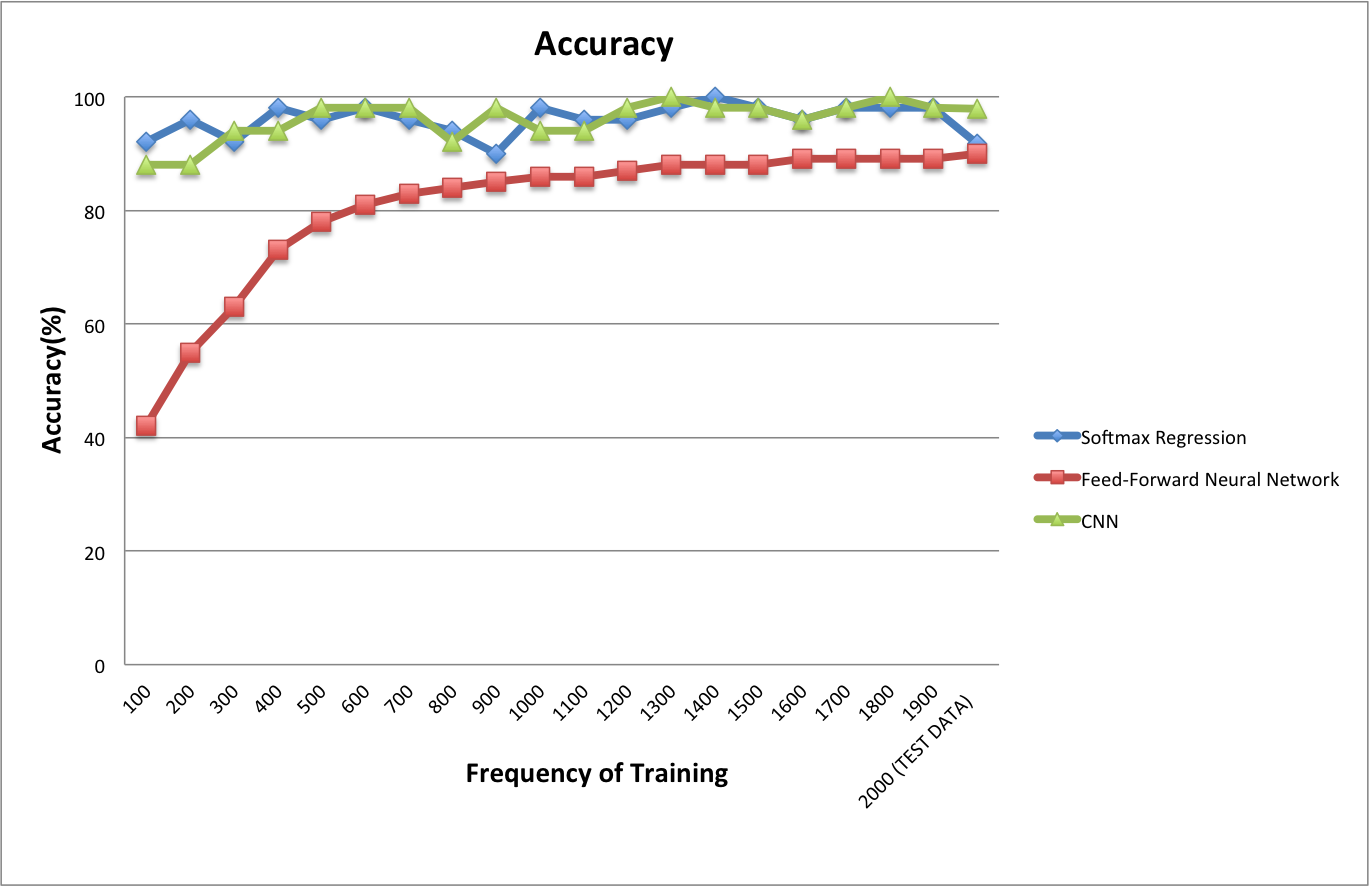
\includegraphics[width=0.7\textwidth]{figures/accuracy}
    \caption{Accuracy curve}
    \label{fig:accuracy}
  \end{center}
\end{figure}

\begin{figure}[t!]
  \begin{center}
    % Note how the file extension has been removed from the filename below
    % so that the LaTeX command can automatically pick any supported file format
    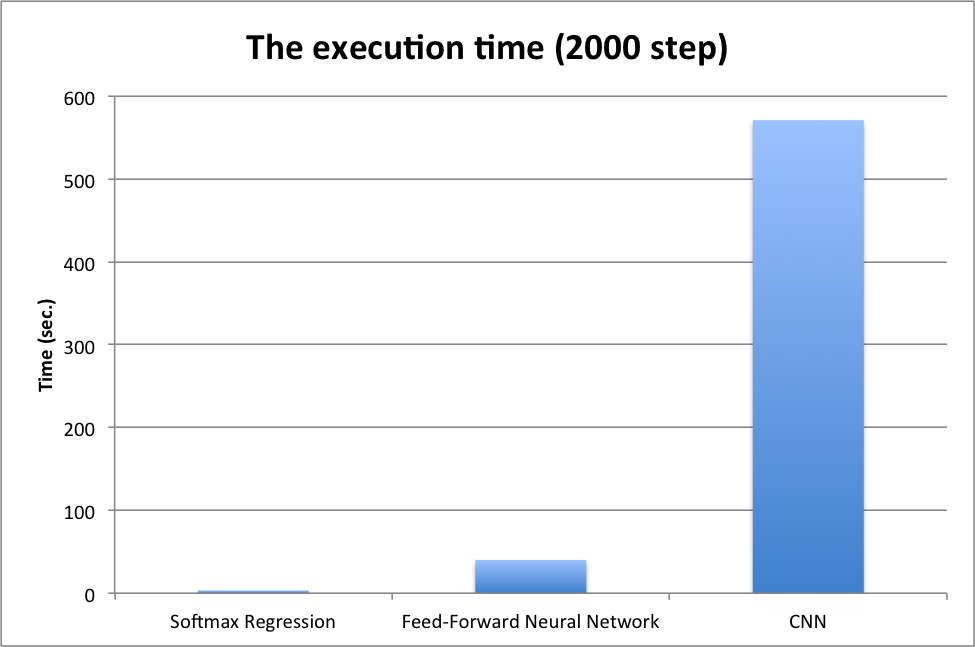
\includegraphics[width=0.7\textwidth]{figures/execution_time}
    \caption{Training execution time curve}
    \label{fig:execution_time}
  \end{center}
\end{figure}

\section{Conclusion}
\label{sec:conclusion}

In this paper, our main work is: first learned related knowledge about machine learning, especially deep learning. 
We learned three types of deep learning approaches could be used in our self-driving car project, evaluated their
performance by analysis the accuracy of them.

According to our experimental result, we think the CNN is the best choice of our project, the main reason is the high accuracy
and can keep the high accuracy on the test data set. Although the training time of CNN is obviously higher than other
approaches, we can still accept it since in our project we are gonna to use a server with 2 NVIDIA GPUs.
With the help of those GPUs, we are able to speed up the training significantly.

%============================================================


\bibliographystyle{plain}
\bibliography{cs-seminar}

\end{document}
